\documentclass[a4paper,10pt]{article}

\usepackage[hidelinks]{hyperref}
\usepackage{float}

% Lingua
\usepackage[utf8]{inputenc}
\usepackage[italian]{babel}

% Margini
\usepackage{geometry}
\geometry{a4paper, top=3cm, bottom=3cm, left=3cm, right=3cm}
\setlength{\parindent}{0pt}

% Grafica e formule
\usepackage{graphicx}   % per immagini
\usepackage{amsmath, amssymb} % per formule matematiche
\usepackage{hyperref}   % per link
\usepackage{caption}    % per didascalie

\title{Relazione progetto\\ Programmazione a Oggetti\\  Biblioteca virtuale}
\author{Giuliano Banchieri, 2101081 \\ Chiara Grossele, 2101063}
\date{Anno accademico 2024/2025}

\begin{document}

\maketitle
\tableofcontents
\newpage


\section{Introduzione}

Il programma PaoLibrary che abbiamo sviluppato è pensato per permettere di gestire una libreria multimediale di oggetti, utilizzando il linguaggio di programmazione C++ e il framework QT. Il programma permette di gestire la visualizzazione, ricerca, modifica, creazione ed eliminazione di elementi della libreria di vario tipo. È possibile inoltre salvare la propria libreria o caricarne una già esistente in file JSON/XML.

La visualizzazione avviene tramite una interfaccia intuitiva dotata di menù a tendina per operazioni di salvataggio/caricamento, una barra di ricerca, una serie di filtri e una griglia su cui vengono visualizzati gli elementi.Oltre alla vista generale sulla libreria, in cui si vedono soltanto titolo e immagine degli oggetti, è possibile visualizzarne i dettagli semplicemente cliccando su di essi.

Il cuore del programma è costituito dalla classe Library che gestisce tramite la sua QList le operazioni sopra descritte da effettuare sugli oggetti  e la sua derivata LibraryModel che fa da intermediario con l'interfaccia grafica.

\section{Modello logico}
Il modello logico della biblioteca si divide in 3 parti: la gerarchia delle classi rappresentanti gli elementi, la libreria che li raccoglie e la gestione dei file JSON/XML.
In cima alla gerarchia delle classi item, vi è la classe astratta AbstractItem che rappresenta un oggetto generico della libreria e contiene i campi comuni a tutti gli elementi. Da questa classe derivano altre due classi astratte PhysicalItem e DigitalItem. Queste due classi si estendono ulteriormente nelle seguenti classi:
\begin{itemize}
    \item Art
    \item Book
    \item la classe astratta Video, da cui derivano le classi:
        \begin{itemize}
            \item Movie
            \item Series
        \end{itemize}
    \item Videogame
\end{itemize}

Esistono poi le classi JsonManager e XmlManager a cui la classe Library delega il compito di tradurre un file JSON/XML esistente in una lista di AbstractItem da caricare nella libreria.
Per poter effettuare delle operazioni legate ad un tipo specifico, e più complesse delle semplici getAttribute e setAttribute appartenenti alle classi item, abbiamo implementato il visitor pattern tramite una serie di classi visitor che su chiamata accept(visitor), eseguono ognuna il proprio compito con metodi sviluppati specificatamente per ogni classe concreta di item.
Questi visitor sono stati utilizzati in particolare per far visualizzare correttamente all'utente interfacce di analisi e creazione di elementi specifiche per l'elemento richiesto. 
\begin{figure}
    \centering
    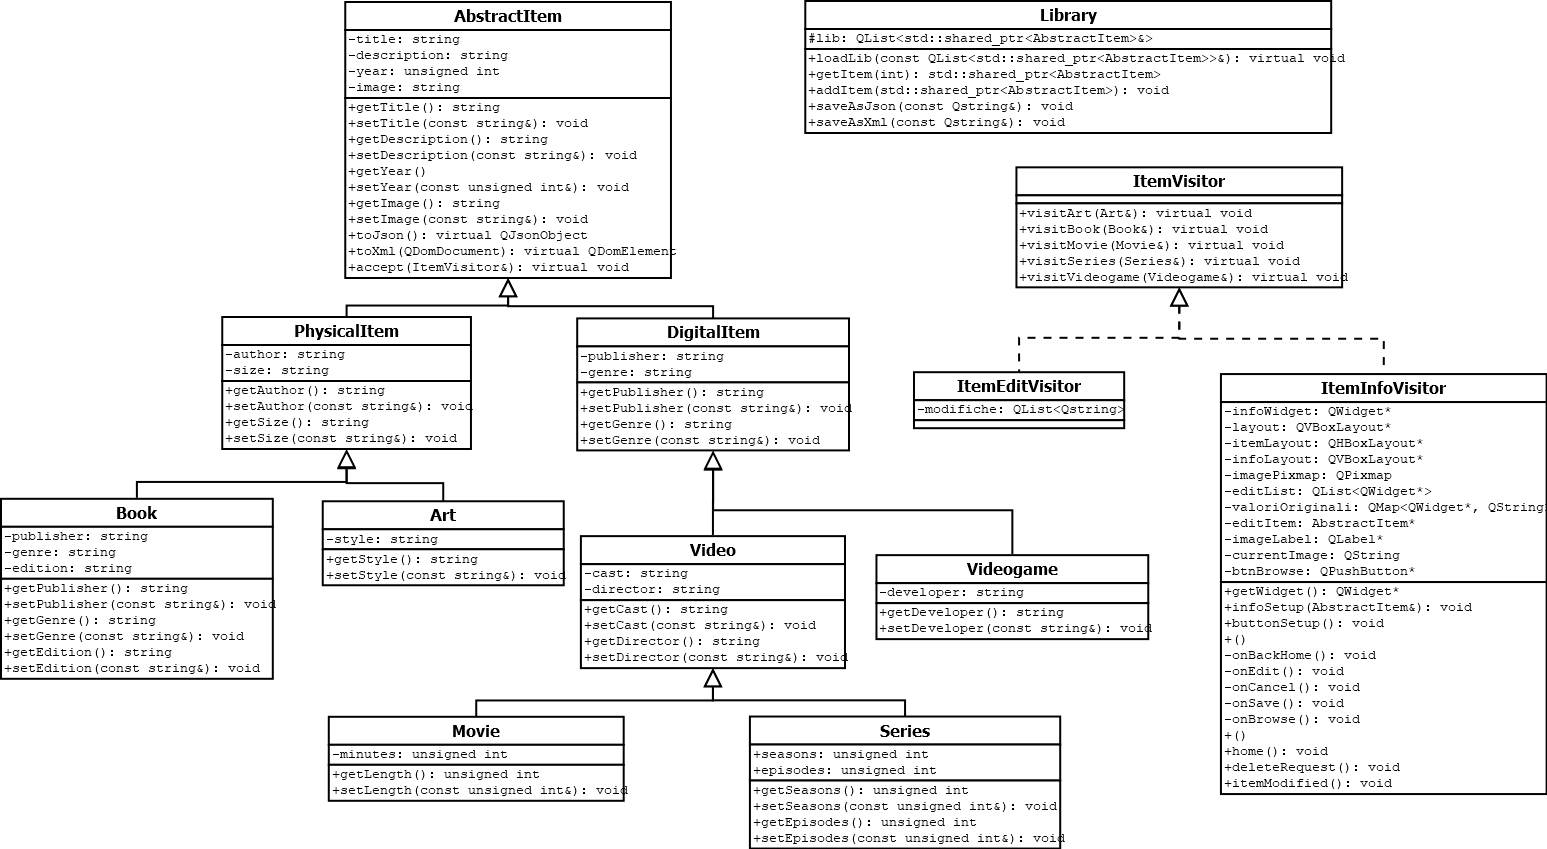
\includegraphics[width=1\linewidth]{PaoLibrary_dia.png}
\end{figure}
\section{Polimorfismo}
In questo progetto il polimorfismo viene utilizzato in modo significativo tramite l'implementazione del design pattern Visitor, che permette di effettuare operazioni complesse che debbano variare dinamicamente in base al tipo concreto di oggetto su cui vengono effettuate.

Abbiamo sfruttato questo pattern per la costruzione di widget personalizzati adibiti alla visualizzazione dettagliata degli elementi della libreria e per la modifica di questi.
\\

Per creare il widget con i dettagli degli oggetti, abbiamo creato il visitor ItemInfoVisitor, derivato dalla classe astratta ItemVisitor e da QObject. Questo visitor è dotati di alcuni metodi aggiuntivi rispetto ai vari visitItem, necessari per la creazione e il posizionamento delle parti di interfaccia comuni necessarie ad ogni oggetto (i campi per gli attributi comuni di AbstractItem e i bottoni per interagire con l'oggetto). Dopo la creazione del widget da visualizzare e il suo setup inziale, in base al tipo di oggetto da cui è stato chiamato, il visitor costruisce le QLabel e QLineEdit necessarie e le inizializza con i dati ottenuti tramite i metodi item.getAttribute().
Una volta costruito il widget richiesto, ItemInfoVisitor lo consegna, tramite il metodo getWidget(), alla MainWindow che lo aggiunge al proprio stackedWidget e lo mette in primo piano.
\\

Un altro visitor che abbiamo utilizzato è ItemEditVisitor che viene utilizzato in combinazione con ItemInfoVisitor per modificare l'elemento della libreria in caso di conferma della modifiche effettuate. Quest'ultimo infatti, una volta entrato in modalità di modifica tramite apposito pulsante, si salva i valori originali dei campi per resettare tutto in caso di annullamento delle modifiche e salva in una lista da passare a ItemEditVisitor i campi aggiornati in caso di conferma. ItemEditVisitor prende poi questa lista e imposta gli attributi dell'oggetto in base ai valori aggiornati trovati in essa.



\section{Persistenza dei dati}
I dati della libreria multimediale possono essere salvati in due formati: JSON e XML. 
Naturalmente è possibile anche utilizzare questi formati per caricare una nuova libreria.

Il salvataggio e caricamento di un libreria sono facilmente accessibili all'utente tramite un pratico e intuitivo menù a tendina.
Vengono forniti assieme al progetto i file libreria\_completa.json e libreria\_completa.xml come esempi.

\section{Funzionalità implementate}
Le funzionalià implementate si posso dividere in 2 categorie: funzionali e grafiche
\subsection*{Funzionali}
\begin{itemize}
    \item Gestione di 5 diversi categorie di oggetti multimediali
    \item Possibilità di ricerca e di filtro per categoria
    \item Salvataggio e Caricamento della libreria in file JSON/XML
\end{itemize}
\subsection*{Grafiche}
\begin{itemize}
    \item Scorciatoie da tastiera (salvataggio dei dati, ritorno alla libreria)
    \item Barra dei menù in cima alla finestra
    \item Visualizzazione generica/dettagliata
    \item Navigazione fra schermate tramite interfaccia
    \item Utilizzo di pulsanti e di una finestra di dialogo per favorire la selezione di immagini durante la creazione o modifica degli oggetti
    \item Avviso in caso di tentativo di uscita dopo aver effettuato modifiche non salvate
    \item Richiesta di conferma eliminazione oggetto
    \item Controllo sovrascrittura file JSON/XML già esistenti su linux
\end{itemize}

\section{Rendicontazione ore}
La rendicontazione delle ore previste e di quelle effettivamente svolte è illustrata nella seguente tabella:

\begin{table}[H]
\centering
\begin{tabular}{|l|c|c|}
  \hline
  Attività & Ore stimate & Ore effettive\\ \hline
  Progettazione modello logico & 5 & 8\\
  Sviluppo del modello & 12 & 15\\
  Studio del framework Qt & 5 & 8\\ 
  Sviluppo GUI &20 &20\\
  Test e debug & 5 & 7\\
  Stesura della relazione & 3 & 3\\ \hline
  Totale & 50 & 61\\ \hline
\end{tabular}
\caption{Rendicontazione delle ore}
\label{tab:esempio}
\end{table}
Il monte ore è stato leggermente superato per qualche problema di coordinazione nella prima fase di progettazione e sviluppo del modello e per alcuni imprevisti dovuti ad una mancanza di confidenza col framework Qt.


\section{Suddivisione del lavoro}
La suddivisione delle attività tra i membri del gruppo è illustrata nella seguente tabella:

\begin{table}[H]
\centering
\begin{tabular}{|l|c|r|}
  \hline
  Attività & Studente \\ \hline
  Progettazione modello logico & Entrambi \\
  Sviluppo modello logico & Entrambi \\
  LibraryModel & Banchieri \\
  MainWindow & Entrambi \\
  JSON & Banchieri \\ 
  XML & Grossele \\ 
  InfoVisitor & Grossele \\
  EditVisitor & Banchieri \\
  Test e debug & Entrambi \\ 
  Stesura della relazione & Entrambi\\ \hline
\end{tabular}
\caption{Suddivisione delle attività}
\label{tab:esempio}
\end{table}



\end{document}

